\documentclass[11pt,letterpaper]{article}
\usepackage[lmargin=1in,rmargin=1in,tmargin=1in,bmargin=1in]{geometry}
\usepackage{worksheet}
\usepackage{listings}
\usepackage{color}
\usepackage{graphicx}
\usepackage{wrapfig}
\graphicspath{ {./images/} }
\usepackage{soul}

\definecolor{dkgreen}{rgb}{0,0.6,0}
\definecolor{gray}{rgb}{0.5,0.5,0.5}
\definecolor{mauve}{rgb}{0.58,0,0.82}

\lstset{frame=tb,
  language=Java,
  aboveskip=3mm,
  belowskip=3mm,
  showstringspaces=false,
  columns=flexible,
  basicstyle={\small\ttfamily},
  numbers=none,
  numberstyle=\tiny\color{gray},
  keywordstyle=\color{blue},
  commentstyle=\color{dkgreen},
  stringstyle=\color{mauve},
  breaklines=true,
  breakatwhitespace=true,
  tabsize=3
}

% -------------------
% Content
% -------------------
\begin{document}
\worksheet{Runtime Practice - Solutions}


% Question 1
\problem Orders of Growth. 
\begin{enumerate}[(a)]
    \item Simplify using Big-O Notation: $N^{2} + NlogN + 1000N + 6$
        \pspace
        \textcolor{red}{$\mathcal{O}(N^2)$}
        \newline
        \textcolor{blue}{In asymptotic analysis, we can drop constants so: $1000N \sim N$ and 6 is a constant. At arbitrarily large inputs (N), $N^2$ dominates. Graph the functions above and notice at large n values $N^2$ grows much faster.}
        \pspace
    \item Calculate the following limit:
    $\lim_{n \to \infty} \frac{n^{2}}{2^{n}}$
        \pspace
        \textcolor{blue}{Use L'Hopital's rule (take the derivative of numerator and denominator until limit is solvable) or the Ratio Test.}
        \newline
        \textcolor{red}{$$\lim_{n \to \infty} \frac{n^{2}}{2^{n}} \rightarrow 0$$}
        \pspace
    \item What does the result of the above limit imply about the exponential and polynomial runtimes. 
    \textit{Hint: Is one always greater (grows faster) than the other?}
        \pspace
        \textcolor{blue}{The denominator $2^n$ grows to infinity faster than $n^2$ so the limit above goes to zero.}
        \newline
        \textcolor{red}{Takeaway: Exponential runtimes always dominate polynomials.}
        \pspace
    \item True or False: If function f has $\mathcal{O}(n)$ and $\Omega(1)$, its tight bound is always found by taking the average of n and 1 giving: $\Theta(n)$
        \pspace
        \textcolor{red}{False!}
        \newline
        \textcolor{blue}{Theta bounds are not exactly averages, they are tight bounds used when the upper bound and lower bound runtimes are the same. So in this case, there is no tight bound since $O(n) \neq \Omega(1)$.}
\end{enumerate}
\pspace
\newpage


% Question 2
\problem Iteration
\\ 
What is the runtime of the following functions?
\begin{lstlisting} 
    public static void loopingMore(int[] array) {
        int n = array.length;
        for (int i = 0; i < 3*n*n*n; i++) {
            System.out.println('I love you');
        }
    }
\end{lstlisting}
\textcolor{red}{$\Theta(n^3)$} \newline
\textcolor{blue}{Function prints "I love you" 3*n*n*n times, so runtime becomes $3n^3$ and we can drop the constant.}
\pspace
\pspace

\begin{lstlisting}
    public static void doubleLoopingHalf(int n) {
        for (int i = 0; i < n; i++) {
            for (int j = n; j > 0; j = j / 2) {
                System.out.println('I love you');
            }
        }
    }
\end{lstlisting}
\textcolor{red}{$\Theta(n^2)$} \newline
\textcolor{blue}{Best way to see how this function grows is to try plugging in sample values for n. If the outer for loop runs n times because of the (i++), the inner for loop runs half the amount of times as the outer loop (j = j / 2). The math essentially becomes $(n)(\frac{n}{2}) = \frac{n^2}{2}$, and we drop the constants.}
\pspace
\pspace

\begin{lstlisting}
    public static void weirdLooping(int n) {
        for (int i = 0; i < n; i++) {
            int num = Math.pow(2, i + 1) - 1;
            for (int j = 0; j < num; j++) {
                System.out.println('I love you');
            }
        }
    }
\end{lstlisting}
\textcolor{red}{$\Theta(2^n).$} 
\textcolor{blue}{The loop ends up running the following number of times:}
\newline
\textcolor{blue}{$1 + 3 + 7 + 15 + ... = 1 + (2^2 - 1) + (2^3 - 1) + (2^4 - 1) + ... + (2^n - 1)$}
\textcolor{blue}{The last term dominates as $n \rightarrow \infty$ so the whole sum is dominated by $(2^n - 1) \sim \Theta(2^n)$. We can construct a table for $n=3$ to see how the function behaves and essentially add up our 1s like we did above.}
\textcolor{blue}{
\begin{center}
\begin{tabular}{ |c|c|c|c|c|c| } 
\hline
num & j\textbackslash i & 0 & 1 & 2\\
\hline
1 & 0 & 1 & 1 & 1 \\ 
3 & 1 & . & 1 & 1 \\ 
7 & 2 & . & 1 & 1 \\
7 & 3 & . & . & 1 \\
7 & 4 & . & . & 1 \\
7 & 5 & . & . & 1 \\
7 & 6 & . & . & 1 \\
\hline
\end{tabular}
\end{center}}

\newpage


% Question 3
\problem Recursion
\\
\textit{Practice using the Work Per Layer Summation Formula}
\begin{lstlisting}
    public static void mergeSort(int[] arr, int l, int r) {
        if (l < r) {
            // Compute Middle Index
            int m = (l + r) / 2
            
            mergeSort(arr, l, m);
            mergeSort(arr, m+1, r);
            
            merge(arr, l, m, r); // Runs in linear time 
        }
    }
\end{lstlisting}
\begin{center}
    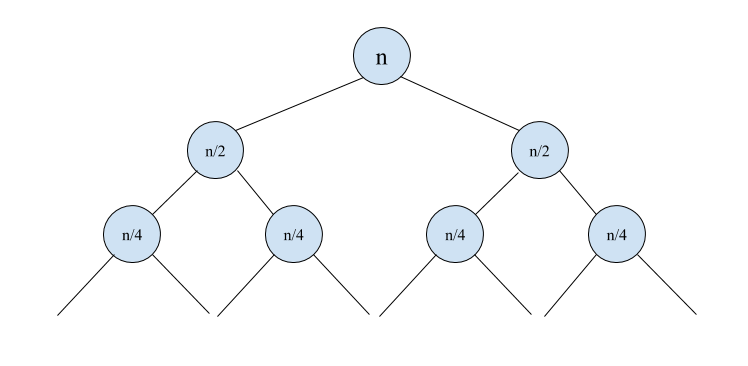
\includegraphics[scale=0.4]{images/mergeSort.png}    
\end{center}

\textcolor{blue}{
Let k be the height/level of the tree (where the root is at k=0).
\newline
\newline
$\frac{work}{node} = \frac{n}{2^k}$ Work is halved at each level
\newline
\newline
$\frac{nodes}{layer} = 2^k$ Nodes double every time 
\newline
\newline
$height = log(n)$
\newline
Height can be seen intuitively by realizing the tree above is balanced and complete and there is a branching factor of 2. It can also be calculated mathematically by calculating how many levels it takes to get to the base case which we can assume is 1: 
$$\frac{work}{node} = \frac{n}{2^k} = 1$$
$$n = 2^k$$
$$log_2(n) = log_2(2^k) = klog_2(2) = k$$
$$k = log_2(n) = log(n)$$
\newline
}
\textcolor{red}{Total Runtime (sum of nodes per layer) = $\sum_{k=0}^{log(n)}\frac{work}{layer}$ = $\sum_{k=0}^{log(n)} 2^k(\frac{n}{2^k})$ = $\sum_{k=0}^{log(n)} n$ = \hl{$\Theta(nlogn)$}}

\newpage
\begin{lstlisting}
    public static void thinTree(int n) {
        if (N <= 1) {return;}
        else {
            thinTree(2);
            thinTree(n / 2);
        }
        
    }
\end{lstlisting}
\begin{center}
    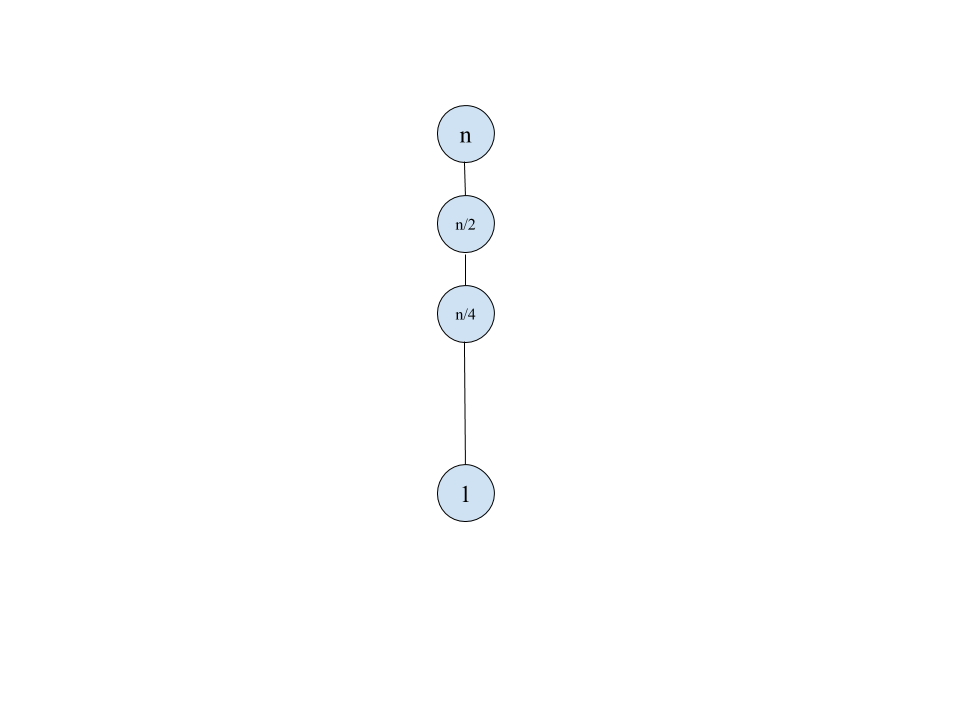
\includegraphics[scale=0.35]{images/thinTree.png}    
\end{center}

\textcolor{blue}{
There are two recursive calls the first one does not add any additional work because the work it does it constant regardless of input size. The work comes from the second recursive call that halves the input at each call. 
\newline
\newline
$\frac{work}{node} = constant$ 
\newline
\newline
$\frac{nodes}{layer} = 1$
\newline
\newline
$height = logn$ As per derivation in the previous question 
\newline
\newline
}
\textcolor{red}{Total Runtime (sum of nodes per layer) = $\sum_{k=0}^{log(n)}\frac{work}{layer}$ = $\sum_{k=0}^{log(n)}1$ = \hl{$\Theta(logn)$}}

\newpage
\begin{lstlisting}
    public static void splitter(int n) {
        if (N == 1) {return;}
        else {
            int i = 0;
            while (i < n) {
                i++
                System.out.println(i);
            }
            return splitter(n / 3) + splitter(2n / 3);
        }
        
    }
\end{lstlisting}
\begin{center}
    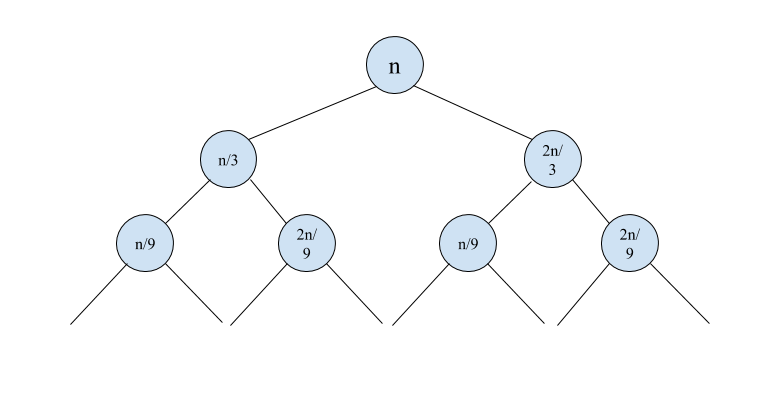
\includegraphics[scale=0.4]{images/splitter.png}    
\end{center}
\textcolor{blue}{Notice each level adds up to n.
\newline
\newline
$\frac{work}{layer} = n$
\newline
\newline
$height = logn$
}
\newline
\newline
\textcolor{red}{Total Runtime (sum of nodes per layer) = $\sum_{k=0}^{log(n)}\frac{work}{layer}$ = $\sum_{k=0}^{log(n)}n$ = \hl{$\Theta(nlogn)$}}


\newpage
% Question 4
\problem Mutual Recursion 
\\
\textit{The following problem has been adapted from Prof. Hug's Sp15 Midterm 2}
\\
\\
State the runtime of each function starting with f1.
\begin{lstlisting}
    public static void f1(int n) {
        for (int i = 0; i < 2*n; i++) {
            System.out.println('Welcome');
        }
    }
\end{lstlisting}
\textcolor{red}{$\Theta(n)$}
\newline
\textcolor{blue}{f1 prints 2n times, leads to linear asymptotic runtime.}
\newline

\begin{lstlisting}
    public static void f2(int n) {
        if (n == 0) { return; }
        f2(n / 3);
        f1(n);
        f2(n / 3);
        f1(n);
        f2(n / 3);
    }
\end{lstlisting}
\textcolor{red}{$\Theta(nlogn)$}
\newline
\textcolor{blue}{f2 is very similar to merge sort but this time with 3 subproblems of a third the size with 2n work per call (see derivations in problem 2).}
\newline

\begin{lstlisting}
    public static void f3(int n) {
        if (n == 0) { return; }
        f3(n - 1);
        f1(16);
        f3(n - 1);
    }
\end{lstlisting}
\textcolor{red}{$\Theta(2^n)$}
\newline
\textcolor{blue}{Every node does the same amount of work per recursive call (which is because f1 is always called with n=16, it is not affected by the n inputted into f3, so there is constant work done per node.  
\newline
\newline
$\frac{work}{node} = 1$
\newline
\newline
$\frac{nodes}{layer} = 2^k$
\newline
\newline
$height = n$
\newline
\newline
$\sum_{k=0}^{n}\frac{work}{layer}$ = $\sum_{k=0}^{n}2^k = 1 + 2 + 2^2 + ... + 2^n = 2^n$ The last term dominates.  
}

\newpage
\begin{lstlisting}
    public static void f4(int n) {
        if (n == 0) { return; }
        f4(n - 1);
        f1(16);
        f1(n);
        f4(n - 1);
    }
\end{lstlisting}
\textcolor{red}{$\Theta(n2^n)$}
\newline
\textcolor{blue}{Same structure as above except work per node is linear.
\newline
\newline
$\frac{work}{node} = n$
\newline
\newline
$\frac{nodes}{layer} = 2^k$
\newline
\newline
$height = n$
\newline
\newline
$\sum_{k=0}^{n}\frac{work}{layer}$ = $\sum_{k=0}^{n}n2^k = n + 2n + 2^2n + ... + n2^n = n2^n$.
\newline}

\begin{lstlisting}
    public static void f5(int n, int m) {
        if (m <= 0) {
            return;
        } else {
            for (int i = 0; i < n; i++) {
                f5(n, m-1);
            }
        }
    }
\end{lstlisting}
\textcolor{red}{$\Theta(n^m)$}
\newline
\newline
\textcolor{blue}{There are n trees each consisting of height equal to m (because of the m-1). The nodes increase by a factor of n at each level. 
\newline
\newline
Total Work = $n + n^2 + n^3 + ... + n^m$. The last term dominates. }



\end{document}